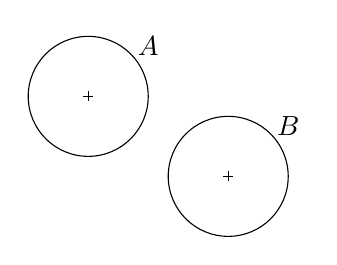
\begin{tikzpicture}[x=1in,y=1in]

	\coordinate (origin) at (0,0);
	\coordinate (I) at (0,0);
	\coordinate (t1) at (30 : 0.8660254038);
	\coordinate (t2) at (-30 : 0.8660254038);
	\coordinate (t1n) at (210 : 0.8660254038);
	\coordinate (t2n) at (150 : 0.8660254038);
	\coordinate (t1s) at (30:2);
	\coordinate (t2s) at (-30:2);
	\coordinate (C) at (0:1);

	\coordinate (B) at (0,0);
	
	\coordinate (A0) at (0*0.05,0);
 	\coordinate (A1) at (1*0.05,0);
	\coordinate (A2) at (2*0.05,0);
	\coordinate (A3) at (3*0.05,0);
	\coordinate (A4) at (4*0.05,0);

	\coordinate (A5) at (5*0.05,0);
	\coordinate (A6) at (6*0.05,0);
	\coordinate (A7) at (7*0.05,0);

	\coordinate (A8) at (8*0.05,0);
	\coordinate (A9) at (9*0.05,0);

	\coordinate (Origin0) at (0, -0*0.6);
	\coordinate (Origin1) at (0, -1*0.6);
	
	\begin{scope} [shift={(0.5, -0.3)}]
		\draw (-0.025,0) -- (0.025, 0);
		\draw (0, -0.025) -- (0, 0.025);
		\draw circle (0.3) node [shift={(0.30, 0.25)}] {$B$};
	\end{scope}

	\begin{scope} [shift={(-0.2, 0.1)}]
		\draw (-0.025,0) -- (0.025, 0);
		\draw (0, -0.025) -- (0, 0.025);
		\draw circle (0.3) node [shift={(0.30, 0.25)}] {$A$};
	\end{scope}

\end{tikzpicture}